% Chapter 3
% Roberto Masocco <robmasocco@gmail.com>
% September 20, 2021

\chapter[Caso di studio: drone autonomo]{Caso di studio: drone autonomo}
\label{chap:Chapter3}
\doublespacing
\fontsize{14}{14}\selectfont
\indent A seguito della discussione portata a termine nei capitoli precedenti circa le nuove soluzioni hardware e software da impiegare per la costruzione di apparati robotici, verrà ora descritto un caso di studio pratico con cui si dimostreranno la validità e l'efficacia di tali strumenti: un drone volante automatico.\\
I task che tale sistema deve svolgere, oltre naturalmente a quelli inerenti il volo in sé, sono specificati nelle regole dell'edizione 2021 del Drone Contest indetto da Leonardo S.p.A. e tenutosi presso la Divisione Velivoli di Leonardo in Corso Francia, Torino. Il prototipo è stato presentato in tale occasione come la proposta del team Asgard Flight Group dell'Università di Roma "Tor Vergata". Il progetto ha coinvolto in tutto cinque tra tesisti e dottorandi afferenti al Dipartimento di Ingegneria Civile e Ingegneria Informatica, i quali sono citati all'inizio di questa Tesi assieme ai loro ruoli e ad un sentito e personale ringraziamento, sotto la supervisione del Prof. Daniele Carnevale. Le regole dell'edizione 2021 del Contest, che costituiscono gli obiettivi operativi del drone, possono essere riassunti come segue:
\begin{itemize}
    \item il drone deve essere in grado di decollare, volare e atterrare autonomamente, orientandosi all'interno di un ambiente indoor di cui è nota a priori la conformazione e la posizione delle piazzole di decollo e atterraggio;
    \item inizialmente il drone deve esplorare l'ambiente, cercando ed individuando dei target mobili costituiti da robot di tipo Roomba che montano un landmark ArUco;
    \item sono noti solo alcuni dei landmark montati sui robot, dunque quando il drone ne individuasse uno sconosciuto, dovrà scattare ed inviare delle fotografie di esso ad una \emph{Ground Control Station} controllata da un operatore;
    \item sulla base di una stringa di punteggi segnata vicino al landmark del robot, dovrà essere decisa una sequenza di atterraggi sulle varie piazzole;
    \item una volta trasmessa la sequenza al drone, esso dovrà eseguire i vari atterraggi, riconoscendo le piazzole sapendone la posizione nella mappa e rilevando i landmark ArUco dipinti su di esse;
    \item durante tutta la durata del volo deve essere possibile inserire il controllo manuale, per ragioni di sicurezza;
\end{itemize}
Per brevità sono stati tralasciati dei dettagli del regolamento inerenti il solo funzionamento della gara. L'obiettivo finale del Contest è chiaramente la massimizzazione del punteggio ottenuto con gli atterraggi, resa non banale dalla presenza nella mappa di ostacoli, rialzi e zone a bassa visibilità.\\
Nel resto di questo capitolo si descriverà più nel dettaglio il robot, partendo dall'hardware e passando poi al software, da quello di più basso livello fino alle logiche di supervisione e comunicazione con GCS ed operatori.\\
Il prototipo realizzato è ritratto in Figura \ref{fig:drone}, mentre una mappa completa del campo di gara è rappresentata in Figura \ref{fig:map}.

\begin{figure}
    \centering
    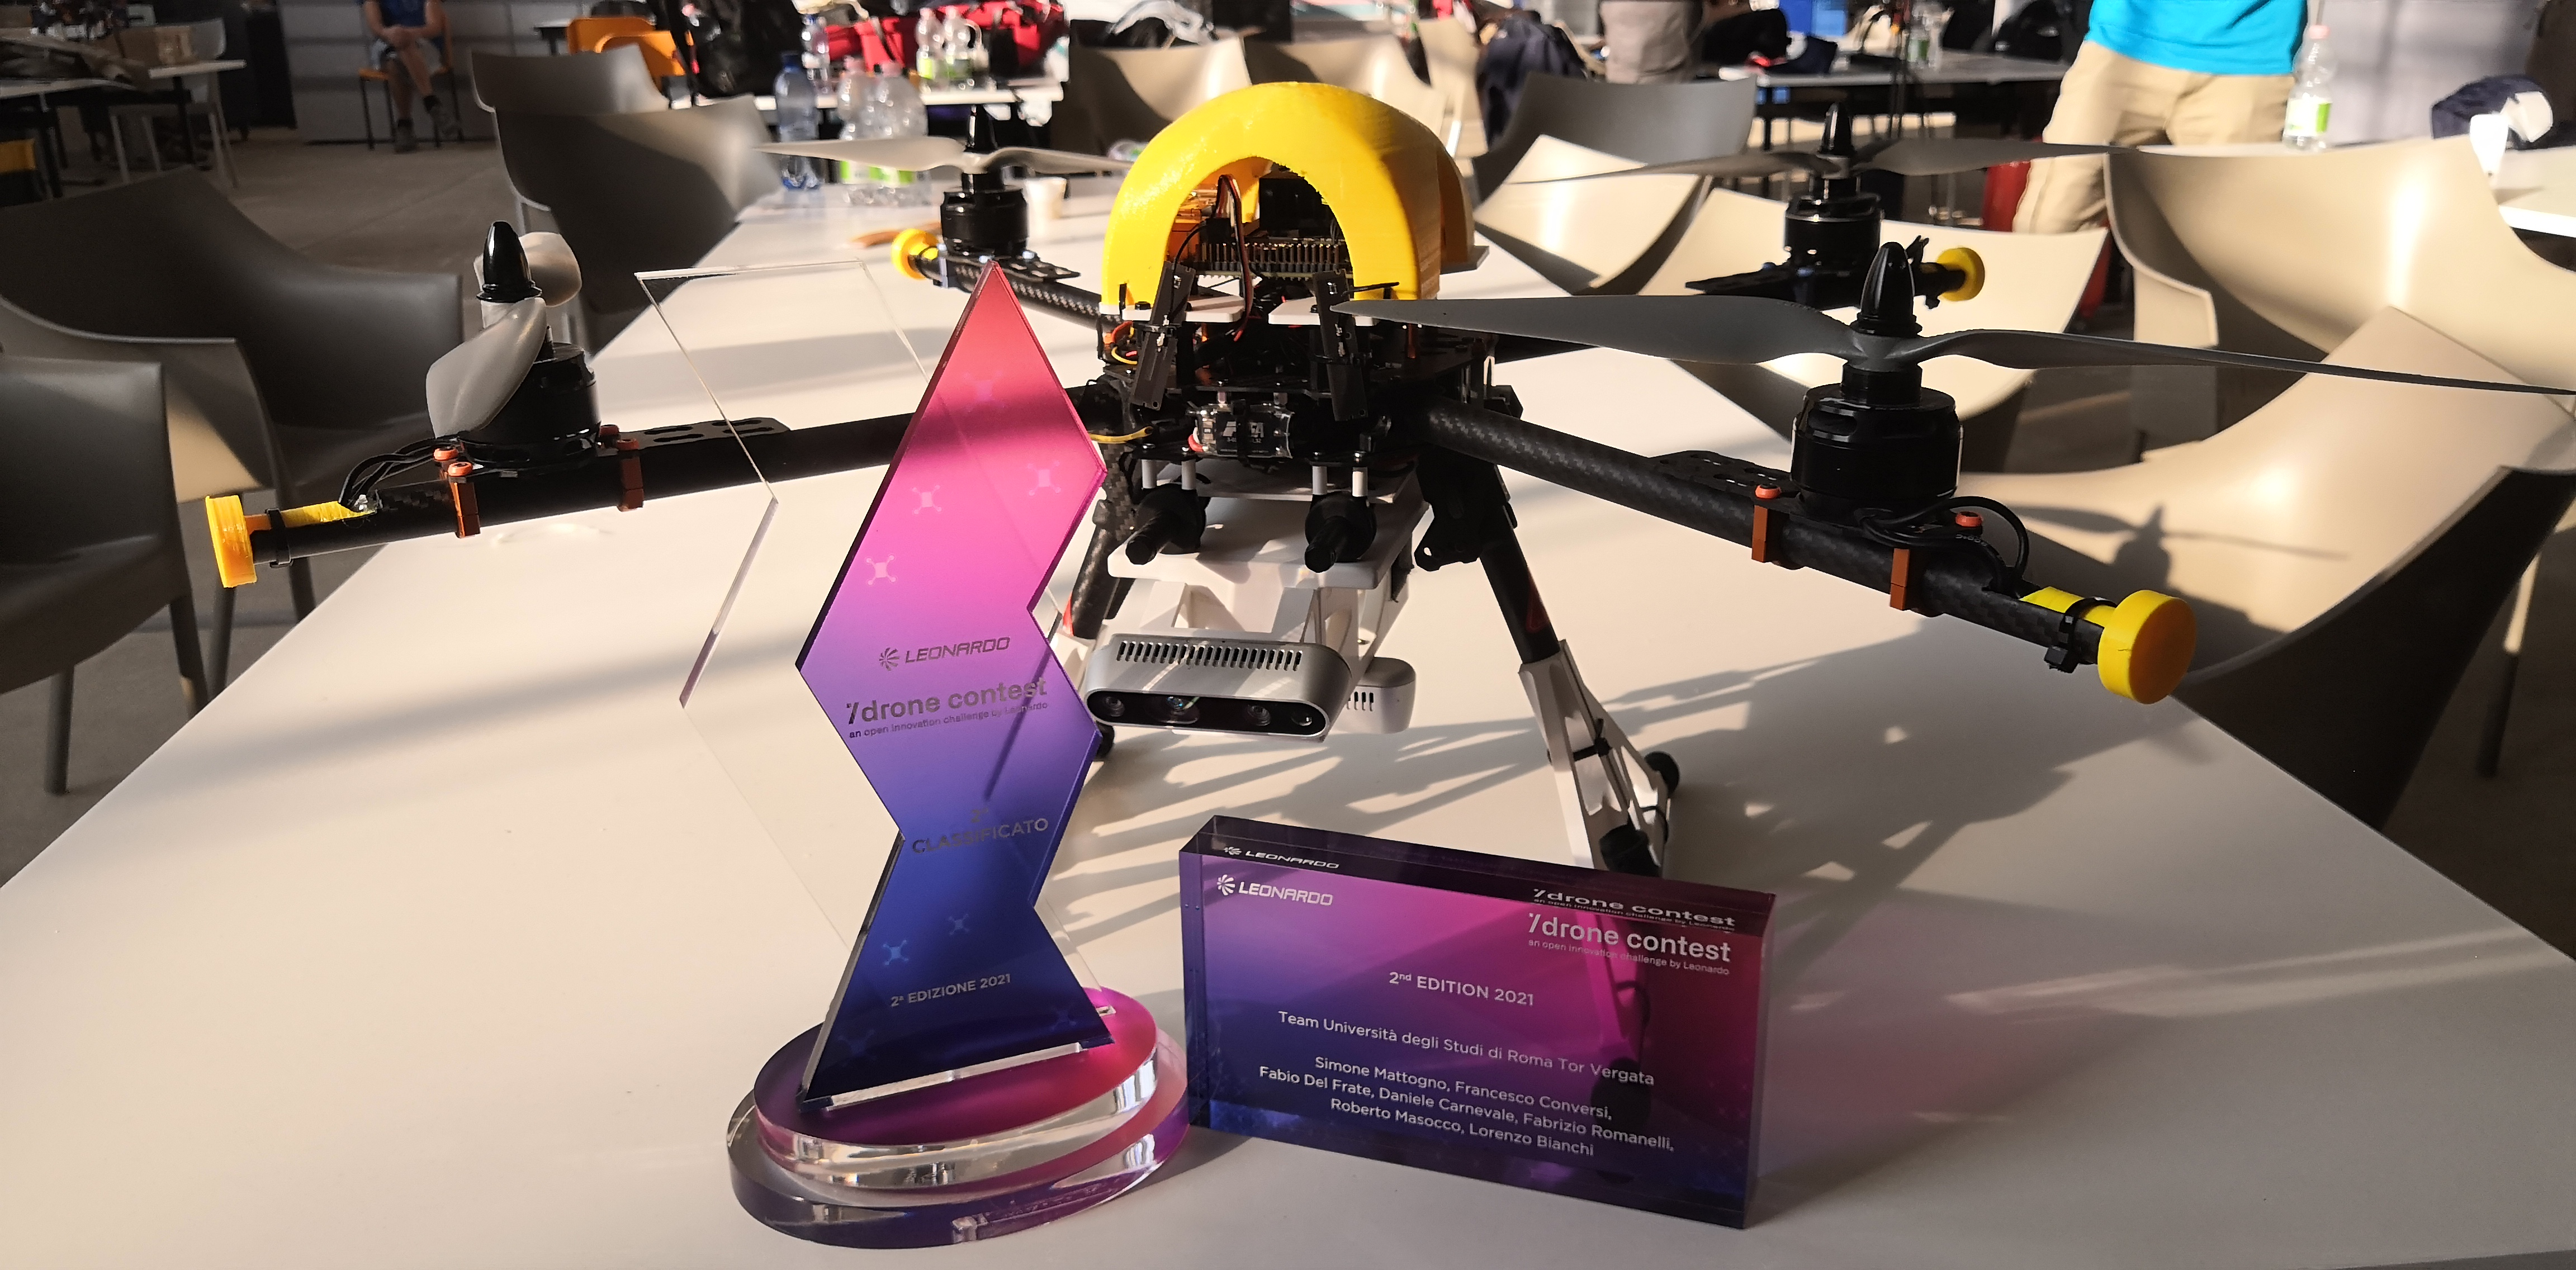
\includegraphics[width=0.8\textwidth]{figs/chapter3/drone.jpg}
    \caption{Prototipo del drone (photo credit: Lorenzo Bianchi).}
    \label{fig:drone}
\end{figure}

\begin{figure}
    \centering
    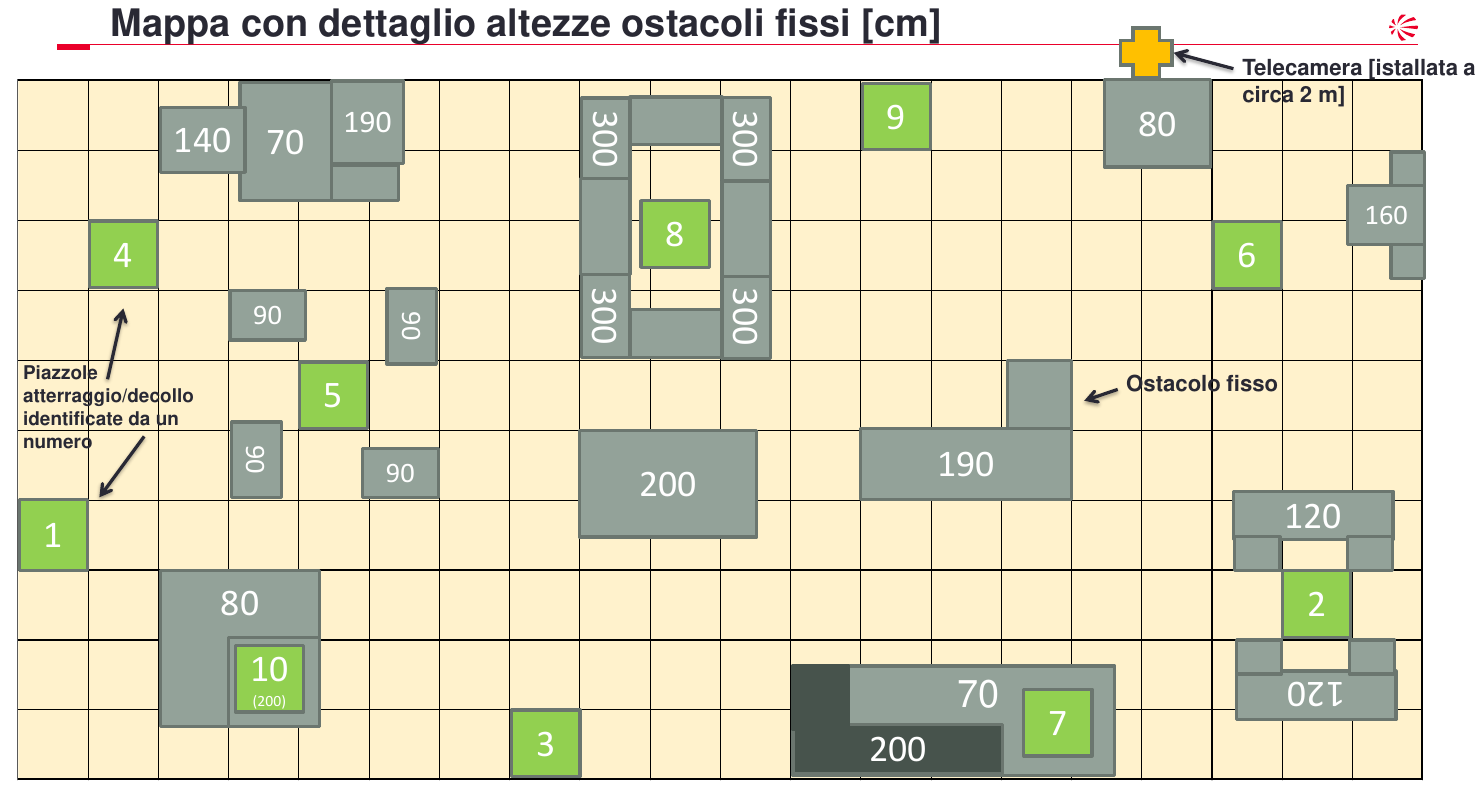
\includegraphics[scale=0.3]{figs/chapter3/campogara.png}
    \caption{Mappa completa del campo di gara.}
    \label{fig:map}
\end{figure}
\clearpage

\newsection{Hardware}
\newsubsection{Frame e motori}
\indent La primissima decisione progettuale ha riguardato la scelta del \emph{frame}, inteso come struttura portante, su cui montare le varie parti. Nell'economia di un drone volante, in special modo autonomo quindi in grado di stabilizzarsi da solo grazie al feedback di vari sensori di bordo, tale struttura deve essere il più leggera e rigida possibile: il primo requisito riguarda naturalmente le prestazioni, l'autonomia e la controllabilità, mentre il secondo ha risvolti sull'accuratezza delle misure di accelerometri e giroscopi. È infatti comune rilevare durante il volo, mediante uno spettrogramma ricavato dai campioni degli accelerometri, delle vibrazioni dovute a vari fattori. Un esempio è mostrato in Figura \ref{fig:flightspec}, relativo ad una prova di volo automatico in pattugliamento. Prendendola ad esempio, si possono notare dei contributi frequenziali predominanti intorno ai 90 Hz, correlati ad altri precedenti nello spettro e di ampiezza minore: sono le armoniche dei motori. Tali vibrazioni non possono naturalmente essere eliminate, e vanno filtrate e reiezionate dal sistema di controllo e stabilizzazione angolare. Alla fine dello spettrogramma (a circa 6:40) si nota quello che sembra un breve urto, che corrisponde al contatto col suolo in fase di atterraggio, in questo caso preciso e privo di rimbalzo. Eventuali altri contributi significativi, in questo caso assenti, sarebbero indice di problemi meccanici o tarature sbagliate del sistema di controllo.\\
Avendo a che fare con questo genere di prototipo però, è necessario anche uno spazio sufficiente ad ospitare i sistemi elettronici, i sensori e le batterie. Per questo la scelta è ricaduta sul frame Tarot 650, realizzato in carbonio e dotato di una piattaforma centrale sufficientemente ampia da permettere il montaggio dell'elettronica di bordo ricavando due livelli superiori e di un pacco batterie in basso. L'intera struttura è stata pensata avendo cura di spostare il meno possibile lungo la verticale il centro di massa aggiungendo carico al frame: montando la batteria in basso questo tende naturalmente a scendere, imprimendo al sistema un comportamento indesiderato simile a quello di un pendolo composto, caratterizzato da oscillazioni difficili da contrastare. A seguito delle diverse prove e dei vari incidenti di percorso, sono state aggiunte dei pezzi volti a irrobustire i punti più fragili e ridurre ancor di più le vibrazioni. Le ulteriori parti meccaniche necessarie sono state modellate con strumenti CAD e stampate in 3D in PLA e TPU: degli esempi particolarmente rilevanti sono mostrati nelle Figure \ref{fig:batpack}, \ref{fig:frontcam}, \ref{fig:canopy}, \ref{fig:triangle}.\\
Per fornire spinta sono stati montati quattro motori brushless T-Motor U3 da 700 W e 700 rpm/V, dotati di eliche da 12 pollici. Essi sono pilotati dal controllore di volo mediante delle ESC\footnote{Electronic Speed Controller.} F35A BLHeli\_32 digitali a 32 bit con protocollo DShot, configurato per trasmissione a 1200 kpbs. Tale protocollo è particolarmente indicato per la trasmissione di comandi agli attuatori dei droni in quanto garantisce bassissima latenza, robustezza agli errori sui bit, e permette di comunicare direttamente con le ESC per configurarle, consentendo ad esempio di impostare il verso di rotazione dei motori senza dover dissaldarne i cavi per invertire le polarità.\vfill\clearpage

\begin{figure}
    \centering
    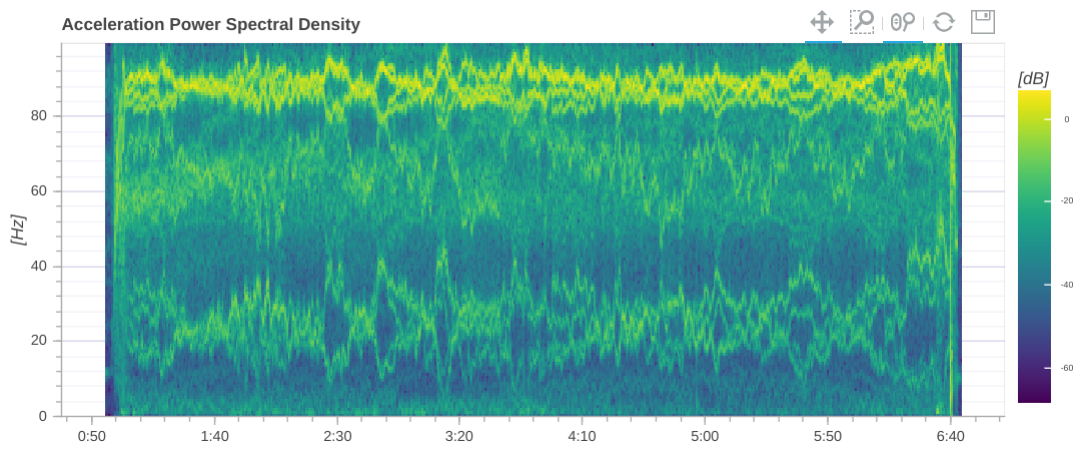
\includegraphics[width=0.9\textwidth]{figs/chapter3/flight_spectro.png}
    \caption{Esempio di spettrogramma ricavato dai dati di un volo automatico.}
    \label{fig:flightspec}
\end{figure}

\begin{figure}
    \centering
    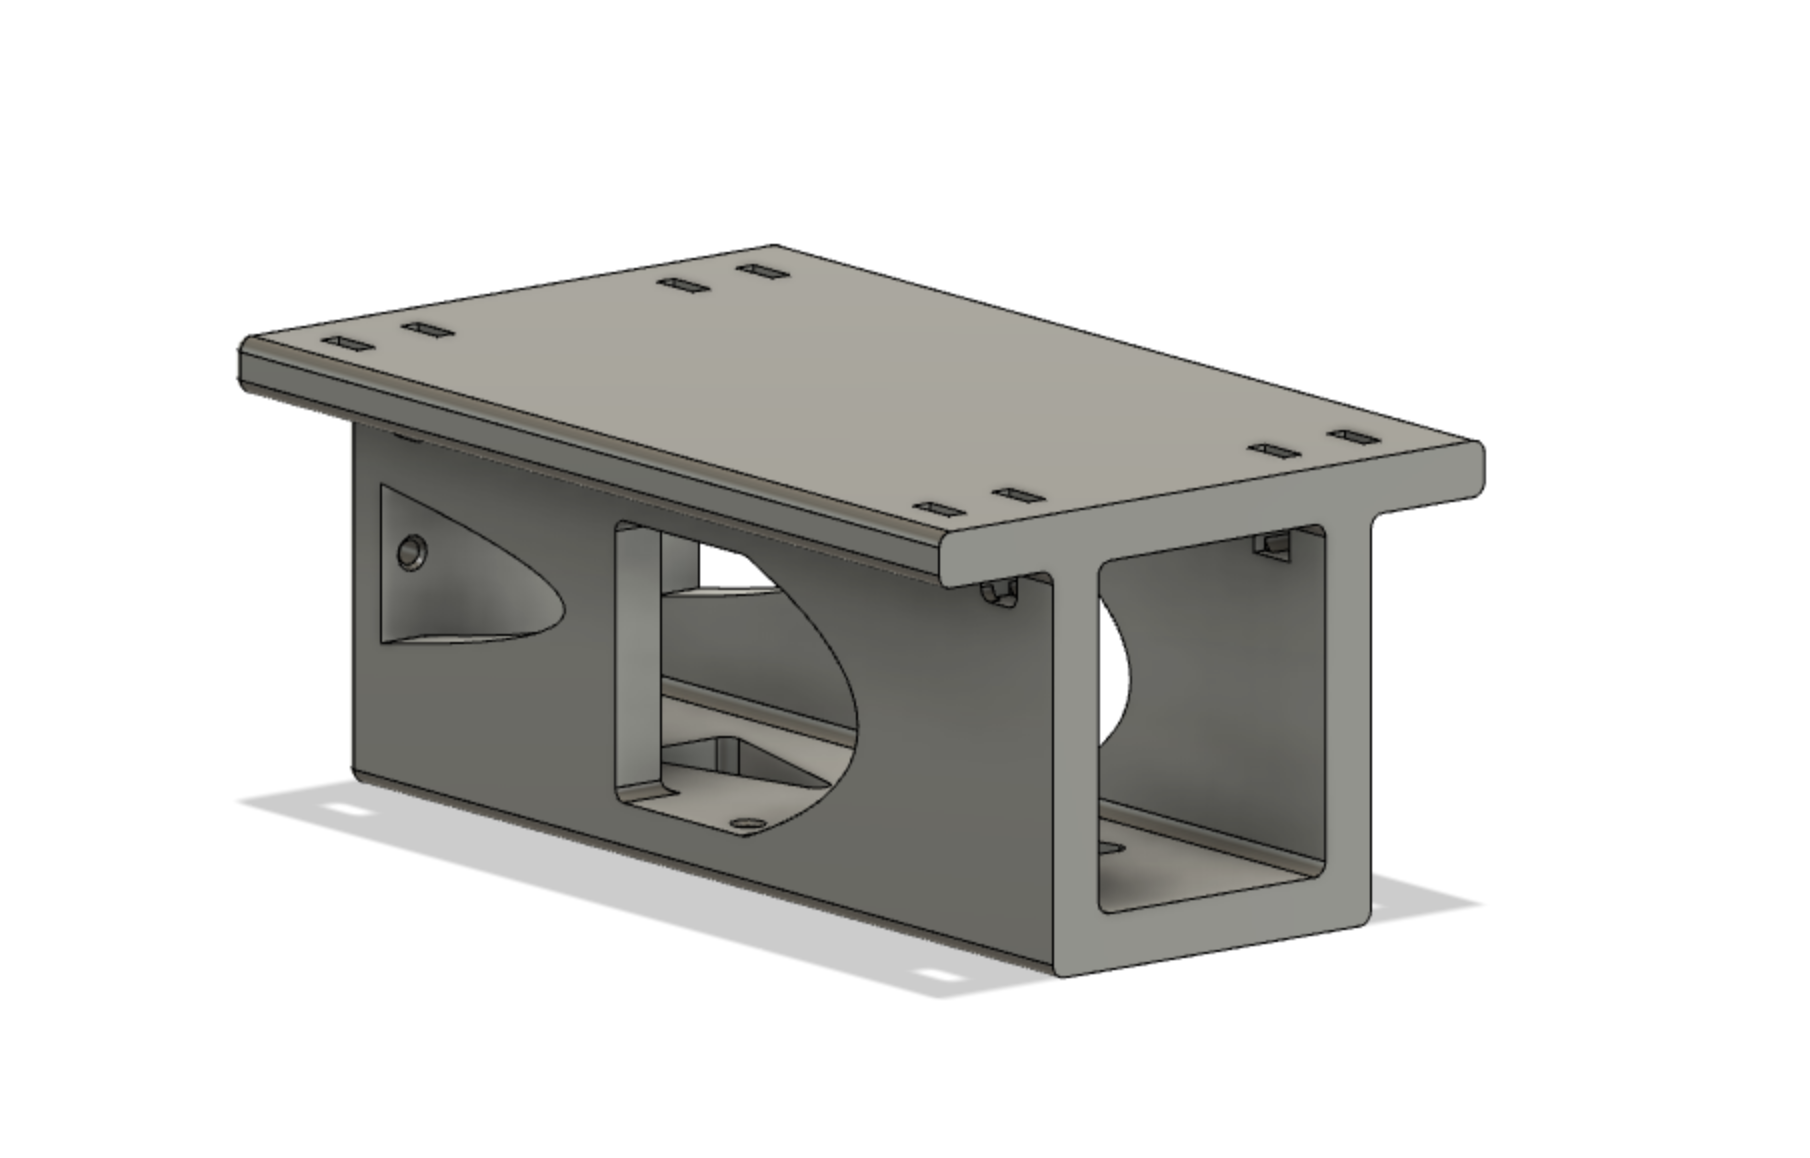
\includegraphics[width=0.9\textwidth]{figs/chapter3/battery-pack.png}
    \caption{Modello CAD del pacco batteria, che funge anche da supporto per la camera inferiore.}
    \label{fig:batpack}
\end{figure}

\begin{figure}
    \centering
    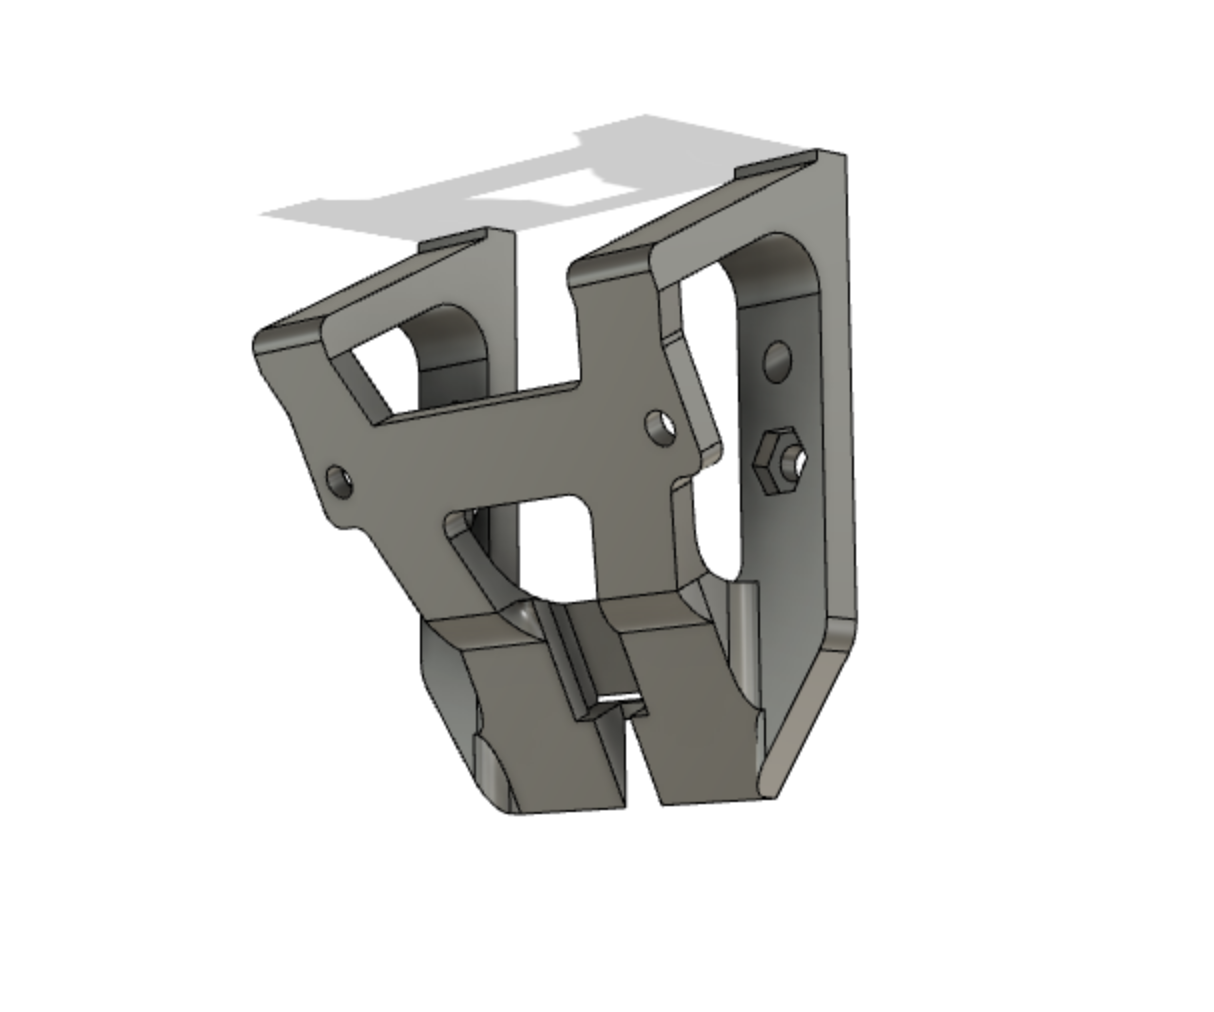
\includegraphics[scale=0.45]{figs/chapter3/camera-holder.png}
    \caption{Modello CAD del supporto della camera frontale, inclinata verso il basso di 26.6°.}
    \label{fig:frontcam}
\end{figure}

\begin{figure}
    \centering
    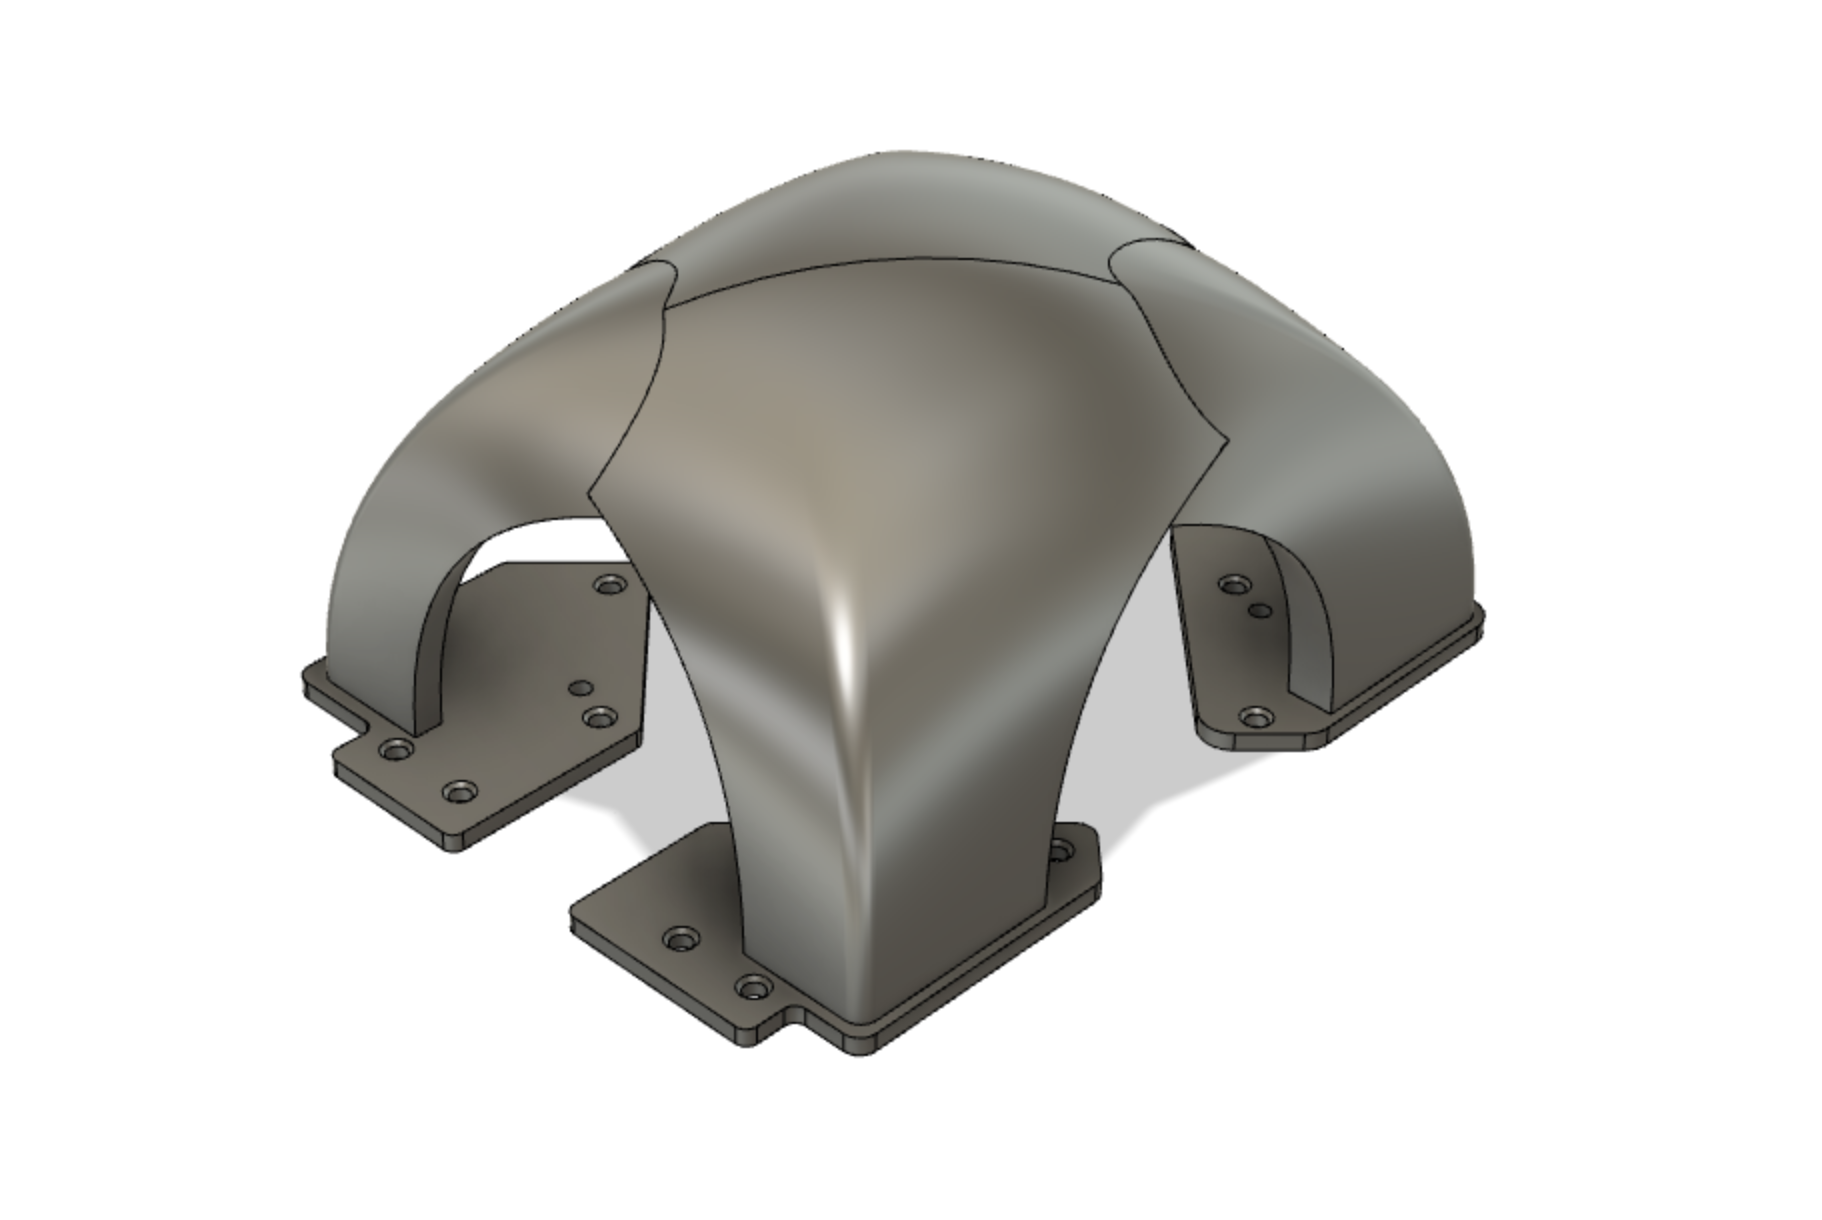
\includegraphics[width=0.9\textwidth]{figs/chapter3/canopy.png}
    \caption{Modello CAD della canopy superiore in TPU, a protezione del computer di bordo.}
    \label{fig:canopy}
\end{figure}

\begin{figure}
    \centering
    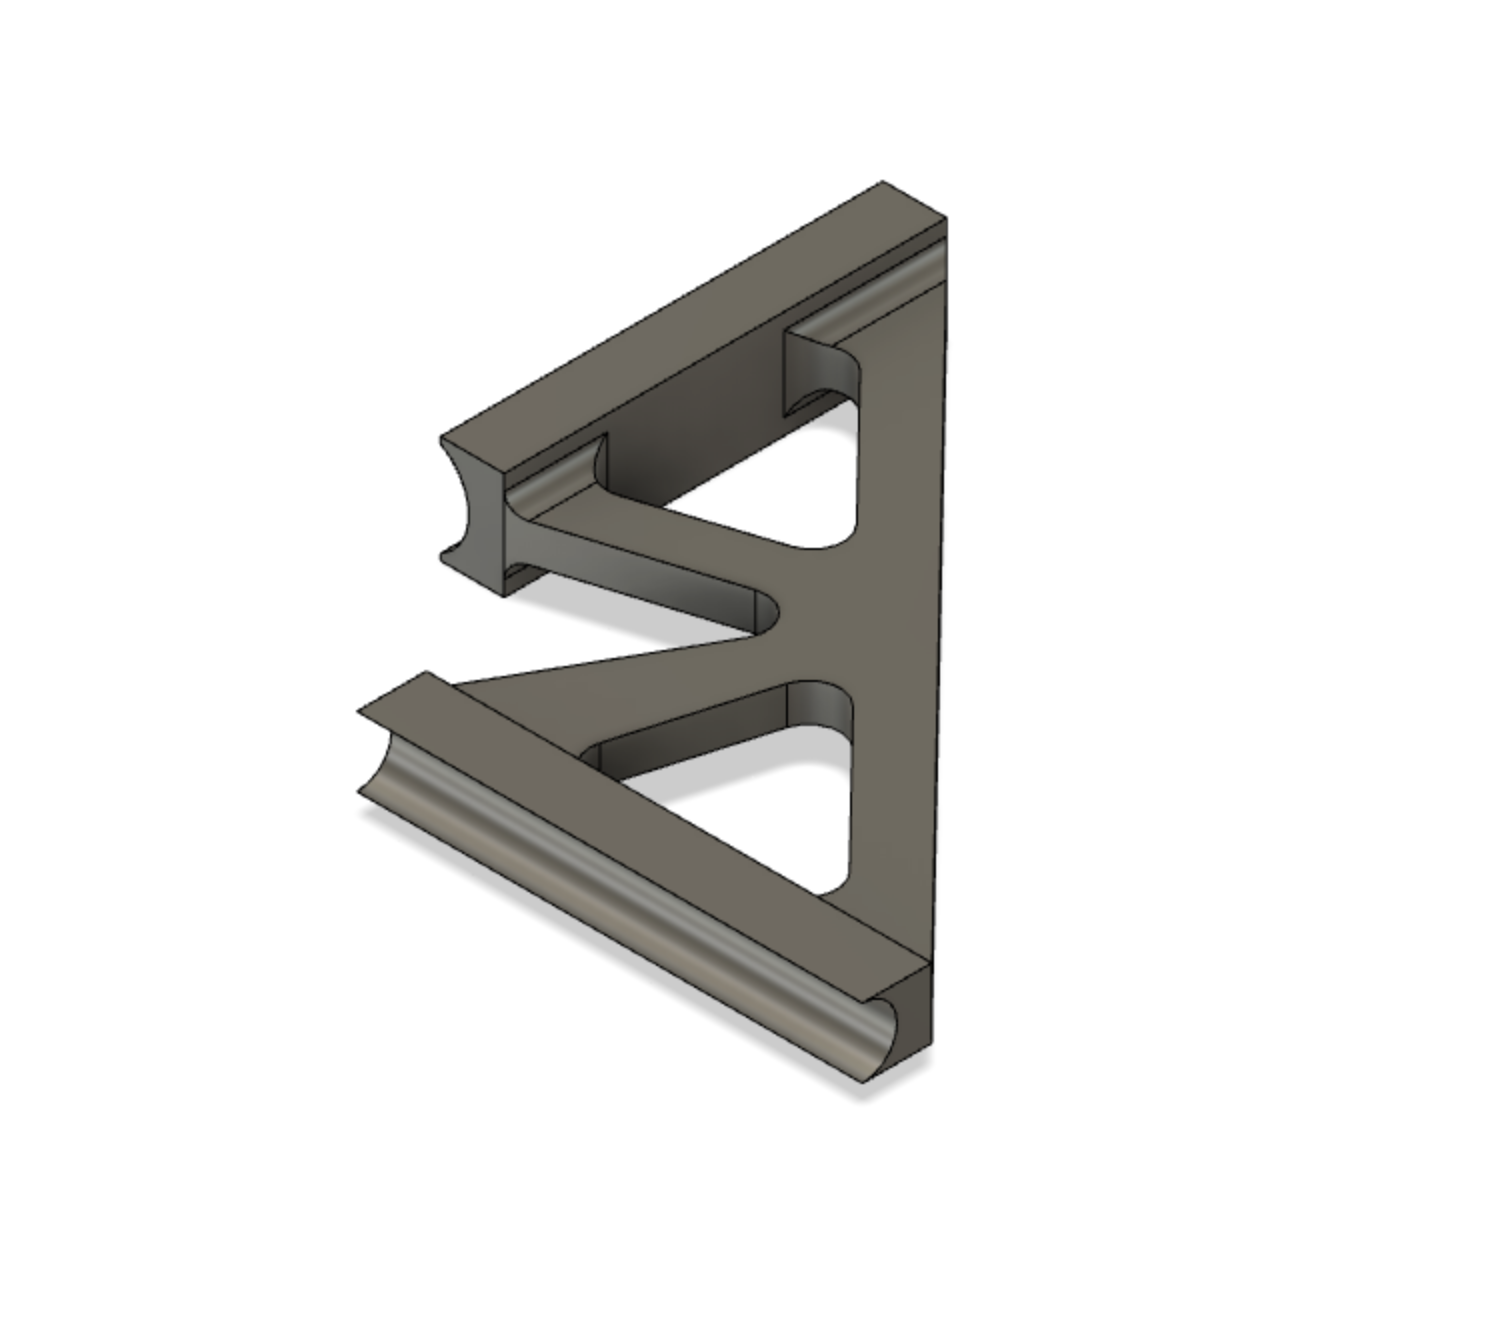
\includegraphics[scale=0.4]{figs/chapter3/triangle.png}
    \caption{Modello CAD del rinforzo triangolare per i carrelli del frame.}
    \label{fig:triangle}
\end{figure}

\newsubsection{Controllore di volo}
\indent La prima parte dell'elettronica di bordo è costituita da un sistema hard real-time\footnote{Con tale locuzione si indica, in genere, un calcolatore elettronico o un controllore numerico per il quale sono specificati una serie di task, ciascuno con delle scadenze temporali precise, e la cui programmazione e realizzazione devono consentire il rispetto tassativo di tali scadenze.} di basso livello, collegato direttamente a sensori e motori, con il compito di localizzarsi in tempo reale e stabilizzare il drone durante le diverse fasi del volo. Per il presente lavoro la scelta è ricaduta sull'Holybro Pixhawk 4, mostrato in Figura \ref{fig:pixhawk}, board compatibile con il firmware open-source PX4 Autopilot\footnote{https://px4.io/}, scritto in C++. Le caratteristiche tecniche principali della board sono riassunte nella Tabella \ref{tab:pix}.
\vspace{1.25cm}
\begin{table}[h]
    \centering
    \begin{tabular}{c|c}
        \textbf{CPU} & STM32F765 32 Bit Arm Cortex-M7 \\
        \textbf{I/O Processor} & STM32F100 32 Bit Arm Cortex-M3 \\
        \textbf{Sensori} & IMU\footnote{Una Inertial Measurement Unit è un sistema avionico che implementa il sistema di navigazione inerziale di un aeromobile. È basato su sensori inerziali, come accelerometri e giroscopi, che permettono un monitoraggio della dinamica di un mezzo in movimento.}, magnetometro, barometro, GPS\\
        \textbf{Interfacce} & UART, GPIO, I2C, SPI, CAN, USB
    \end{tabular}
    \caption{Caratteristiche tecniche del controllore di volo Pixhawk 4.}
    \label{tab:pix}
\end{table}
\vfill\clearpage
La CPU è dedicata all'esecuzione del firmware PX4 sul Real-Time Operating System NuttX\footnote{https://nuttx.apache.org/}, mentre l'I/O processor all'acquisizione dei dati dai sensori e alla gestione delle interfacce di comunicazione verso ESC o altri componenti. Come da regolamento del Contest, il GPS è stato disattivato e scollegato.\\
Alla board è stata collegata una ricevente radio per aggiungere il controllo manuale con l'ausilio di un radiocomando apposito.\\
La caratteristica saliente di questo controllore è la compatibilità con il progetto PX4. Quest'ultimo, essendo open-source, ha consentito di imparare molto circa il funzionamento e il controllo di un drone, ma anche di intervenire sulla configurazione in modo mirato quando necessario, per eseguire tarature o identificare e risolvere i problemi. I principali servizi offerti da questo firmware, che sono stati ritoccati ed impiegati come parte di questo lavoro per mettere in volo il prototipo secondo le specifiche definite dal Contest, sono i seguenti:
\begin{itemize}
    \item possibilità di controllare il velivolo in posizione, velocità, accelerazione o assetto tramite un computer di bordo esterno;
    \item fusione delle misure acquisite da diversi sensori, sia integrati che esterni ed anche temporalmente sfasati, mediante un filtro di Kalman esteso denominato EKF2\footnote{https://docs.px4.io/master/en/advanced\_config/tuning\_the\_ecl\_ekf.html};
    \item link di comunicazione seriale robusto ad alta velocità verso computer di bordo;
    \item filtri dinamici regolabili per rigettare dalle misure vibrazioni spurie o altri disturbi esterni.
\end{itemize}
\vfill\newpage
L'algoritmo di controllo nonlineare implementato da PX4 è descritto in \cite{px4control}, e una sua schematizzazione è mostrata in Figura \ref{fig:px4controller}, con dettagli nelle Figure \ref{fig:px4angular}, \ref{fig:px4attitude}, \ref{fig:px4velocity}, \ref{fig:px4position}. A ciascun livello, ogni controllore prende in ingresso un riferimento da inseguire e calcola un controllo, da applicare al livello successivo oppure direttamente ai motori tramite opportuno mixing. Ai fini del Contest, tra le modalità disponibili sono state impiegate quelle in posizione e in velocità, a seguito di uno studio accurato del sistema e di una precisa taratura dei suoi vari guadagni e saturazioni.\\
Il sistema di comunicazione con il computer di bordo è invece costituito da un bridge tra due DDS, denominato \emph{microRTPS Bridge}, comprensivo di meccanismi di serializzazione e deserializzazione dei pacchetti in transito sul link seriale. Nello specifico, il firmware integra il DDS basico \emph{uORB}, usato anche per le varie comunicazioni interprocesso nel firmware stesso, mentre l'altro lato della comunicazione è basato su \emph{FastDDS}\footnote{https://www.eprosima.com/index.php/products-all/eprosima-fast-dds} di eProsima. Le due parti della comunicazione seriale sono gestite da due software, uno in esecuzione sul controllore di volo e per questo denominato \emph{Client}, ed uno presente sul computer di bordo e chiamato \emph{Agent}.\\
Tale soluzione assicura una comunicazione affidabile, full-duplex e ad alta velocità tra i due componenti, nonché la semplice integrazione con altri middleware quali ad esempio ROS 2. Anche questo progetto è open-source, ed è stato modificato in svariati punti durante questo lavoro al fine di produrre una versione migliore di quella ufficiale, nella quale sono state rilevate gravi mancanze nella gestione di eventuali pacchetti malformati, che potevano portare casualmente al crash del programma. Una schematizzazione dell'architettura di comunicazione è mostrata in Figura \ref{fig:rtpsbridge}.
\vfill\newpage

\begin{figure}
    \centering
    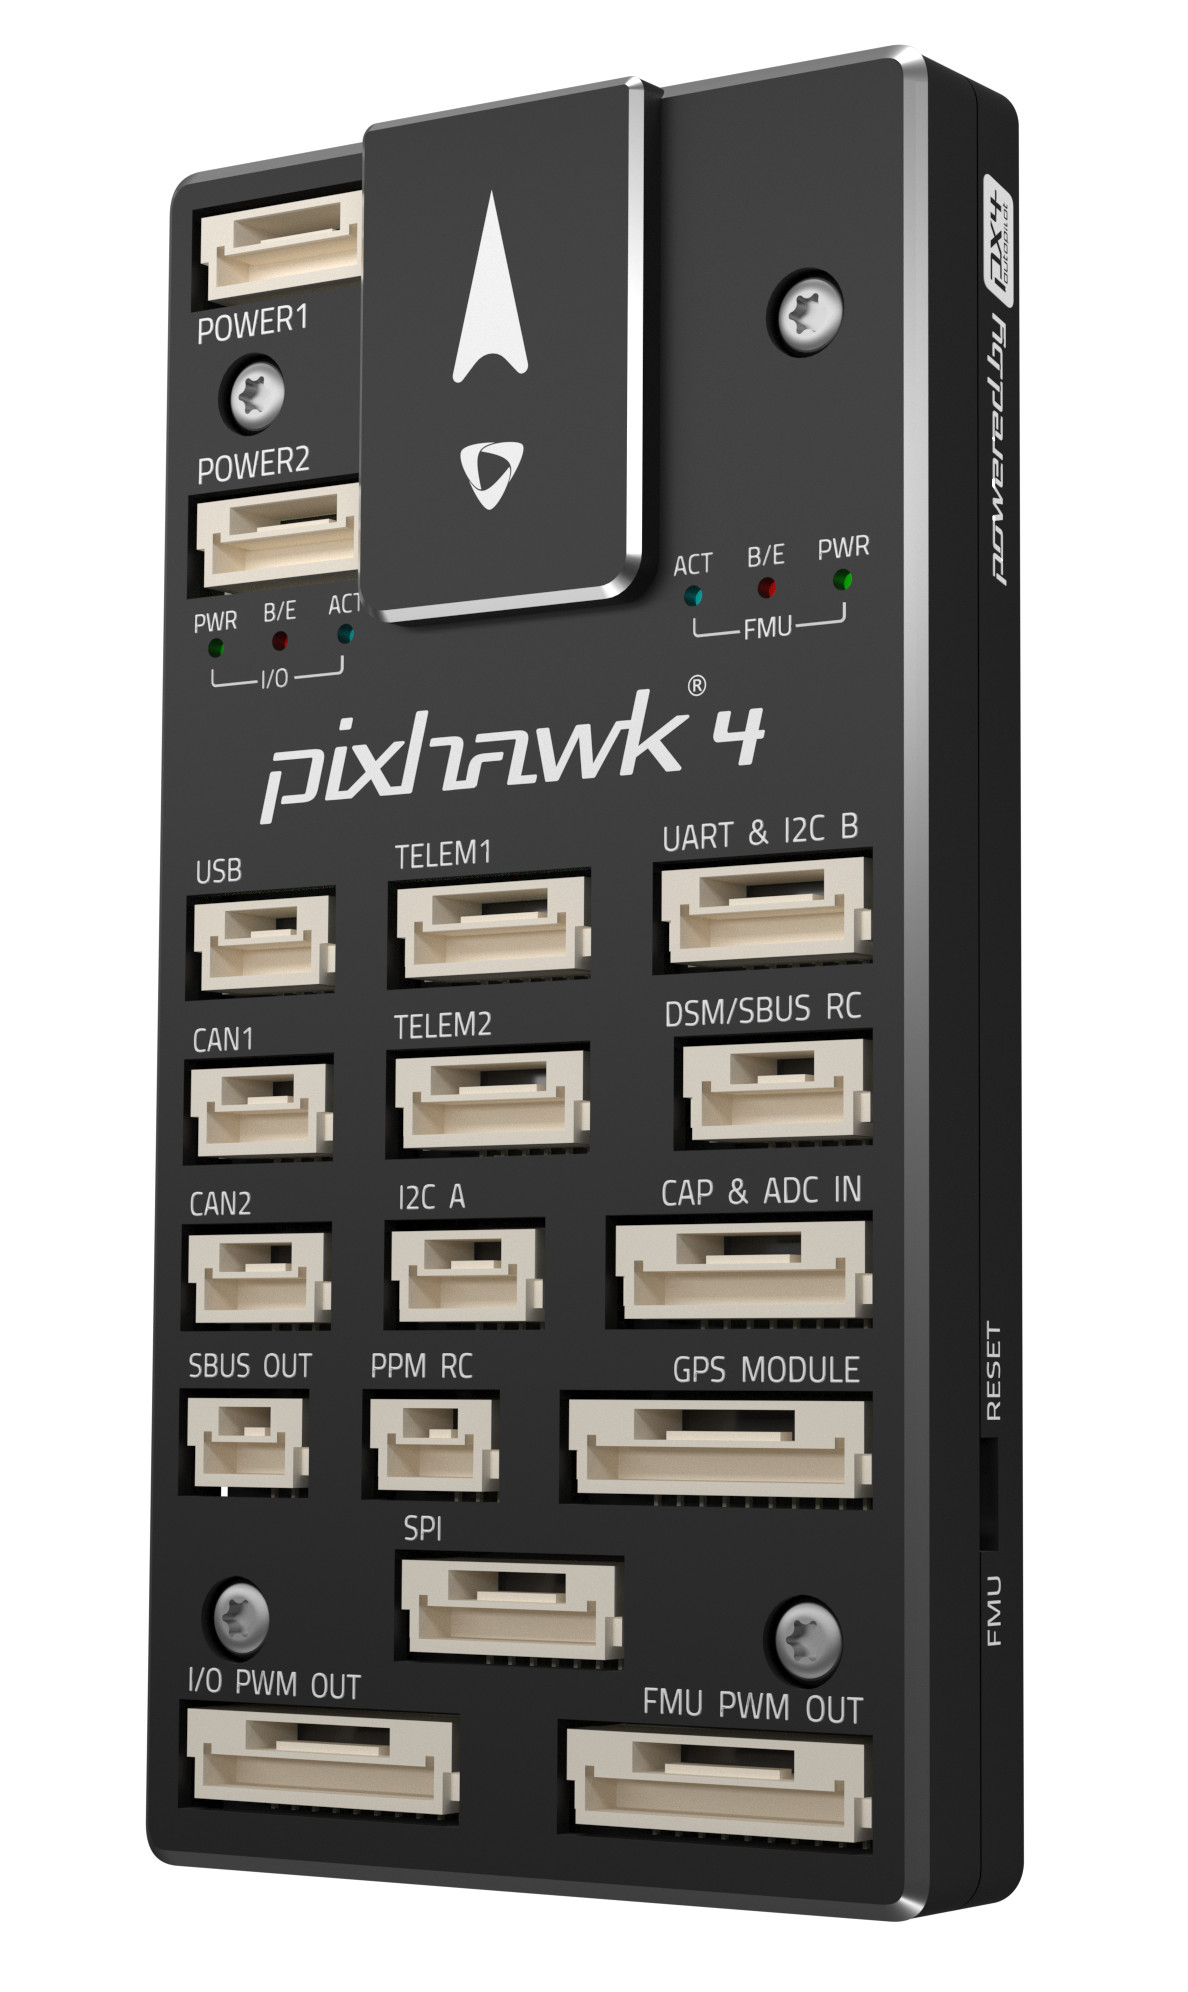
\includegraphics[scale=0.1]{figs/chapter3/pixhawk4.jpg}
    \caption{Controllore di volo Pixhawk 4.}
    \label{fig:pixhawk}
\end{figure}

\begin{figure}
    \centering
    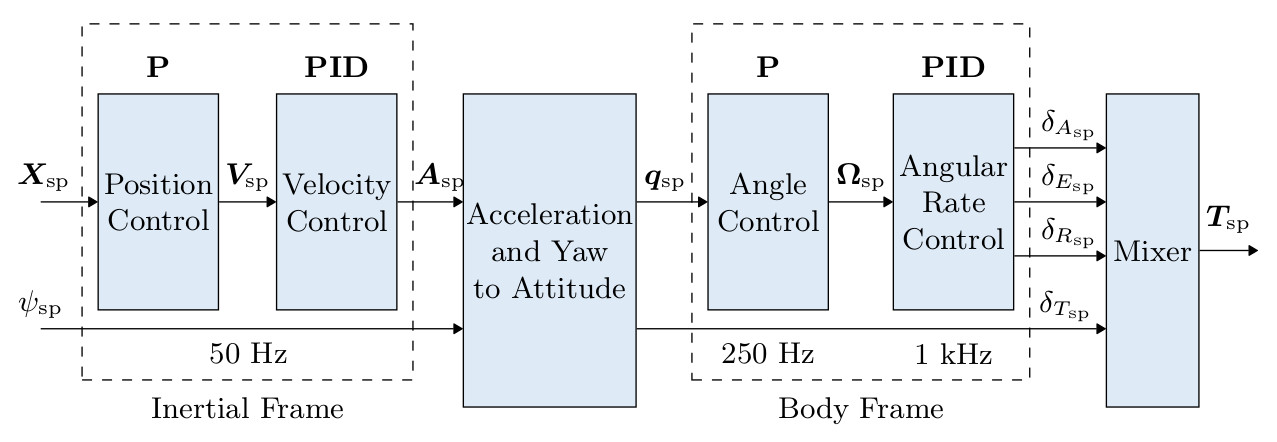
\includegraphics[width=0.9\textwidth]{figs/chapter3/px4-controller.jpg}
    \caption{Schema del controllore di volo multilivello implementato da PX4, con i diversi tempi di campionamento dei vari sottosistemi.}
    \label{fig:px4controller}
\end{figure}

\begin{figure}
    \centering
    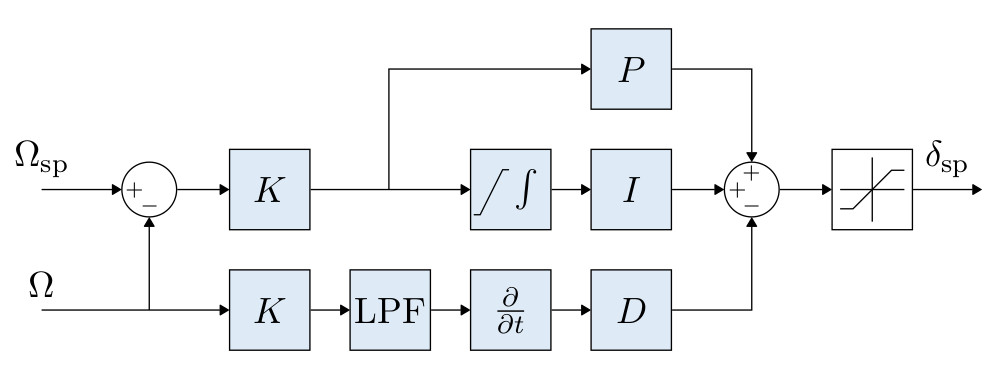
\includegraphics[width=0.9\textwidth]{figs/chapter3/px4-angularcont.jpg}
    \caption{Dettaglio del controllore PID con filtri per la stabilizzazione angolare.}
    \label{fig:px4angular}
\end{figure}

\begin{figure}
    \centering
    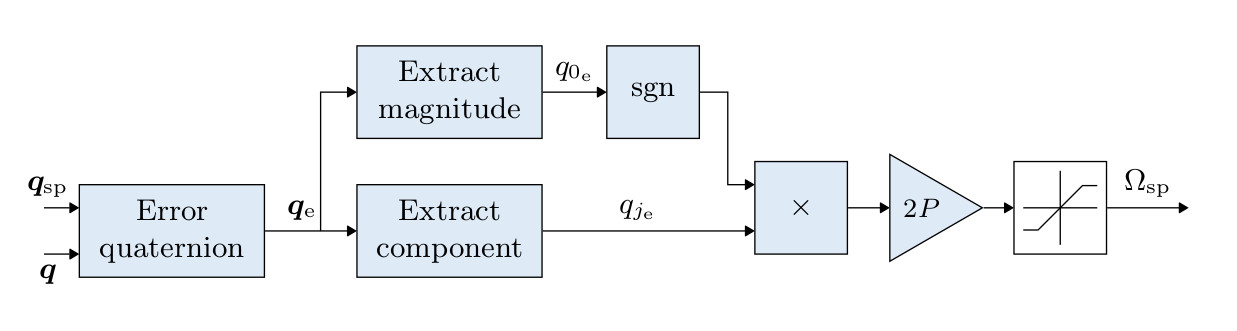
\includegraphics[width=0.9\textwidth]{figs/chapter3/px4-attitude.jpg}
    \caption{Dettaglio del controllore di PX4 per la regolazione dell'assetto basato, sui quaternioni d'orientamento.}
    \label{fig:px4attitude}
\end{figure}

\begin{figure}
    \centering
    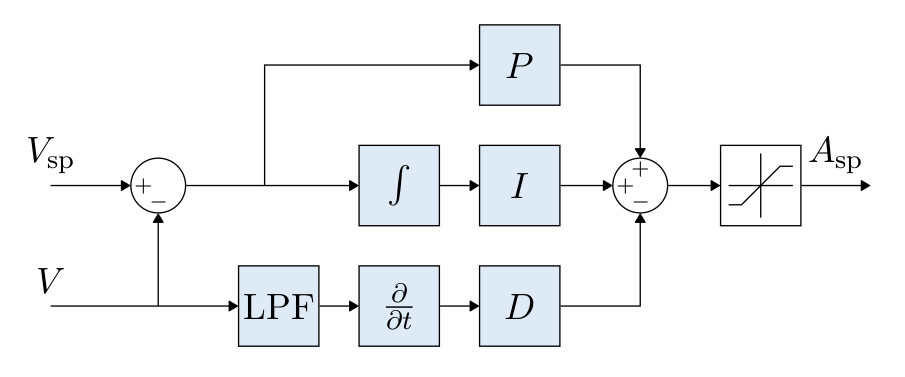
\includegraphics[width=0.9\textwidth]{figs/chapter3/px4-velocity.jpg}
    \caption{Dettaglio del controllore PID con filtri per la regolazione della velocità lineare.}
    \label{fig:px4velocity}
\end{figure}

\begin{figure}
    \centering
    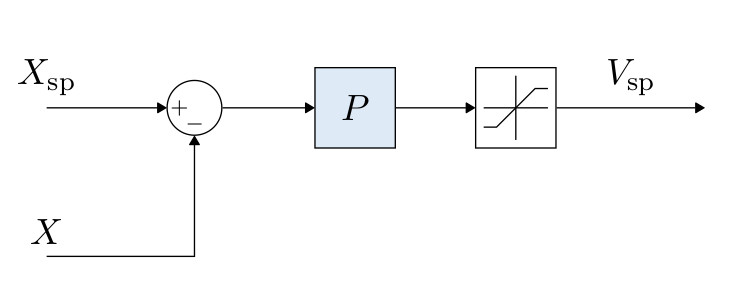
\includegraphics[width=0.7\textwidth]{figs/chapter3/px4-position.jpg}
    \caption{Dettaglio del controllore proporzionale per l'inseguimento della posizione.}
    \label{fig:px4position}
\end{figure}

\begin{figure}
    \centering
    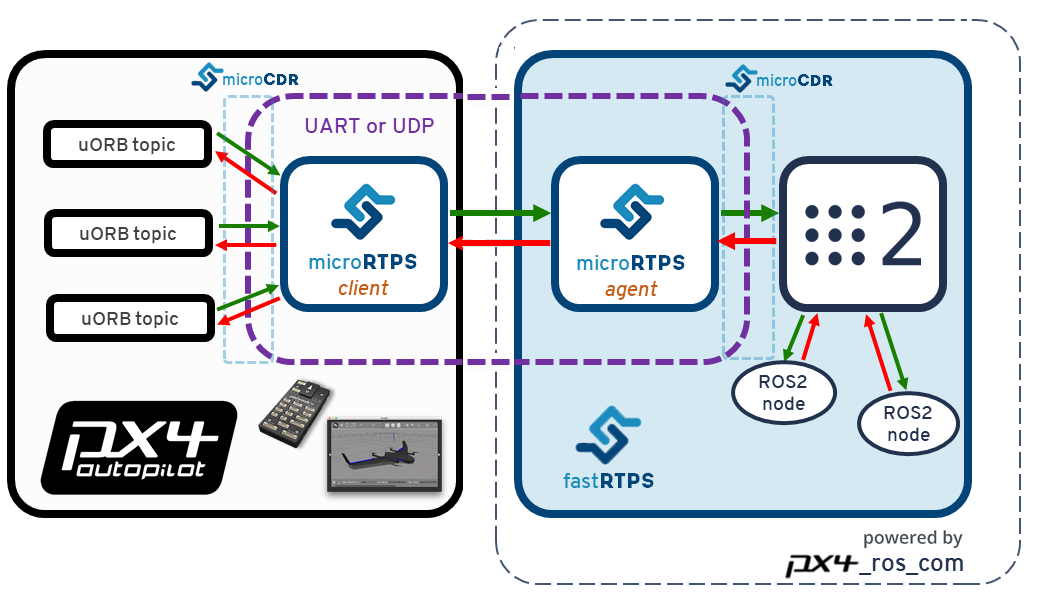
\includegraphics[width=0.9\textwidth]{figs/chapter3/rtps-bridge.png}
    \caption{Architettura del link di comunicazione microRTPS Bridge.}
    \label{fig:rtpsbridge}
\end{figure}

\newsubsection{Fotocamere}
\indent Al fine di riconoscere i target montati sui robot mobili a terra, nonché di localizzarsi nell'ambiente, si sono rese necessarie due fotocamere, montate rispettivamente di fronte e verso il basso. La scelta è ricaduta sulle Intel RealSense D435i (Figura \ref{fig:d435i}), dotate di interfaccia USB 3.1 e vari sensori, dei quali sono stati usati le camere RGB e ad infrarossi per ricavare una mappa di profondità. L'integrazione col resto del software è stata possibile mediante dei driver open-source resi disponibili da Intel.\clearpage

\begin{figure}
    \centering
    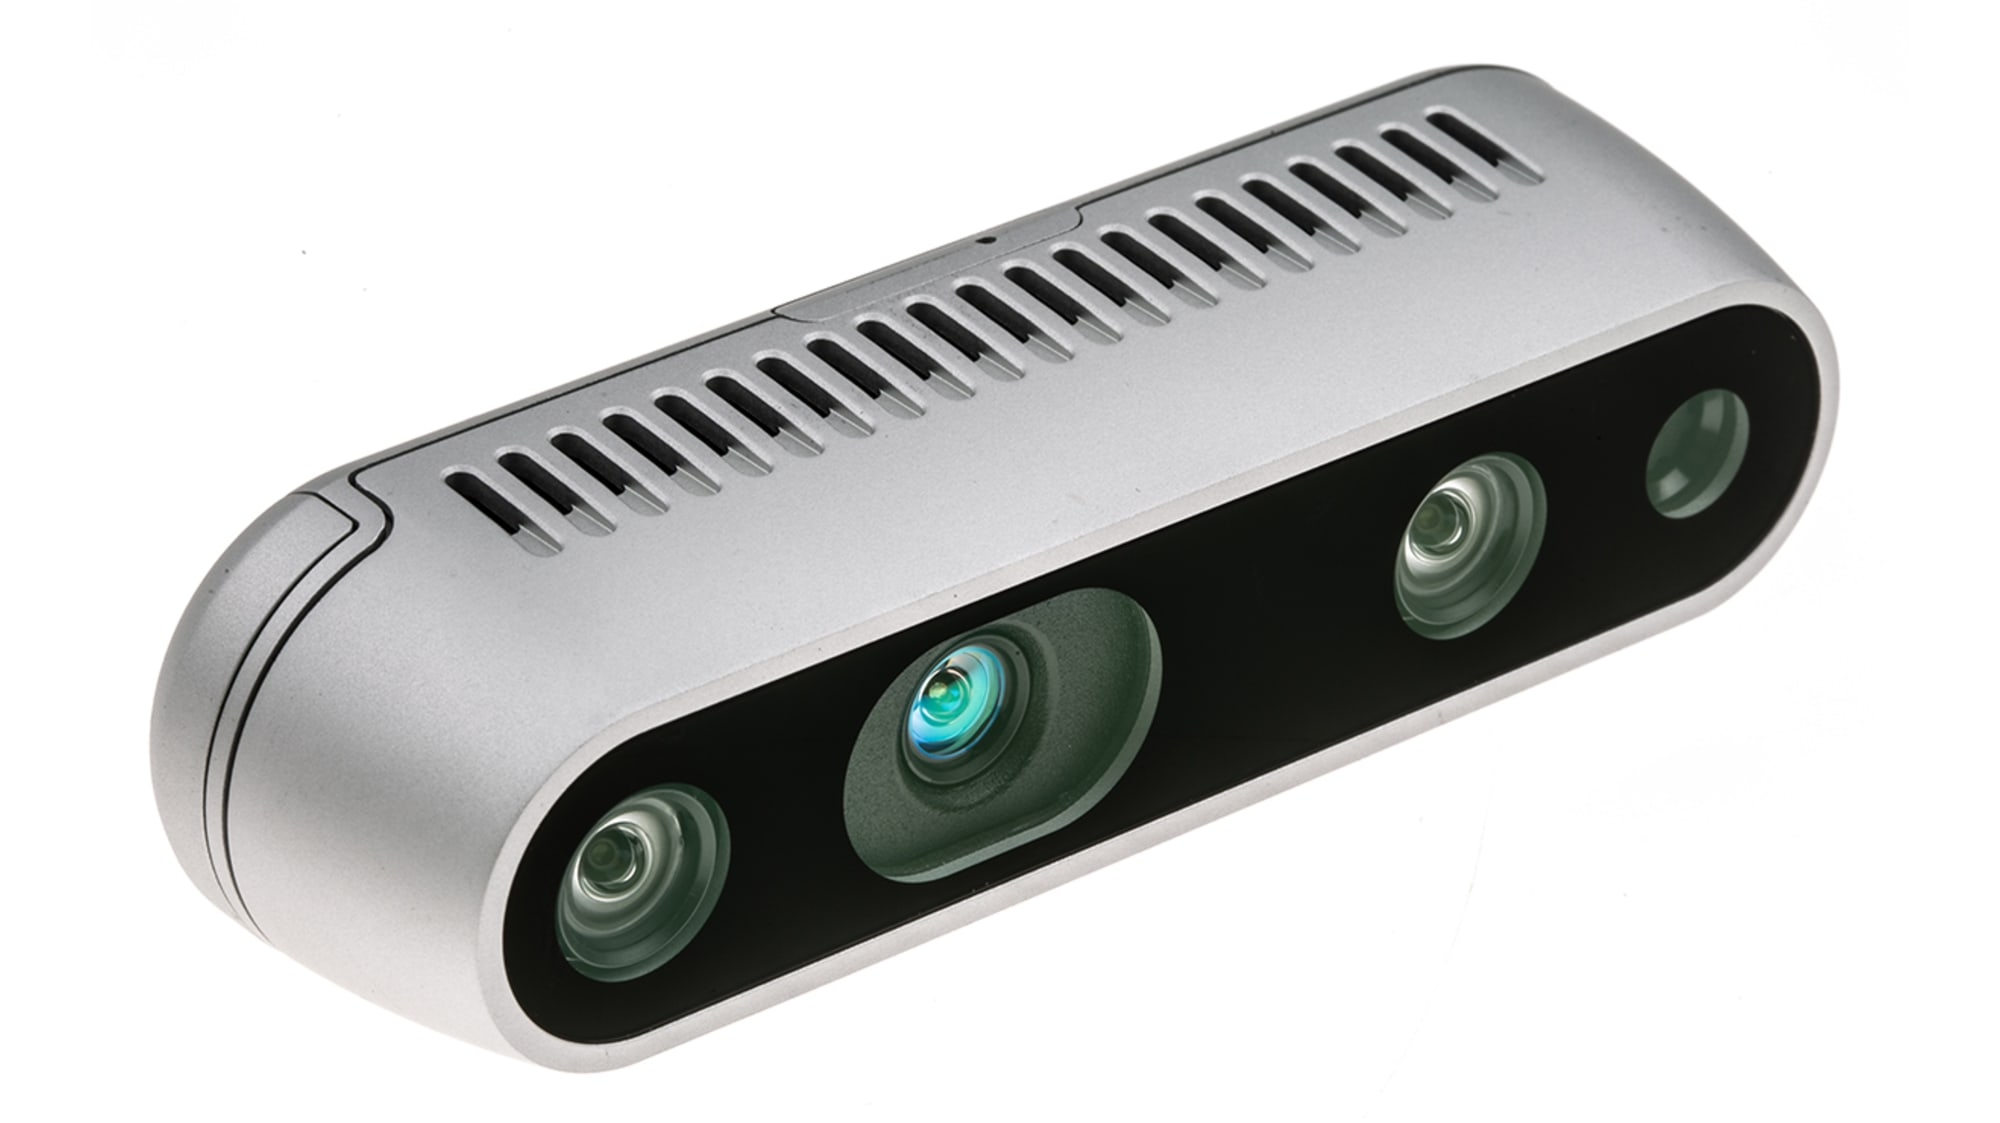
\includegraphics[scale=0.1]{figs/chapter3/d435i.jpg}
    \caption{Intel RealSense D435i stereo depth camera.}
    \label{fig:d435i}
\end{figure}

\newsubsection{Computer di bordo}
\indent La restante parte dell'elettronica è costituita dal computer di bordo. Si tratta in questo caso di un calcolatore di più alto livello, dedicato allo svolgimento dei task più lenti di supervisione e decisione, nonché ai compiti di processamento più onerosi per ottenere una stima precisa della posa locale, implementando le logiche di navigazione e orientamento.\\
Le piattaforme Nvidia Jetson sono state selezionate per questo scopo, in quanto soluzioni SoC altamente efficienti e dotate di svariato hardware integrato, predisposte anche per lo sviluppo di software di qualunque tipo grazie al supporto del sistema operativo Linux. Il modello specifico che è stato adottato è la development board Xavier NX, rappresentata in Figura \ref{fig:nx}. La principale caratteristica di queste soluzioni è l'ampia e varia disponibilità di risorse in un package di dimensioni e consumi contenuti. Le caratteristiche salienti e più utili ai fini del presente lavoro sono riassunte nella Tabella \ref{tab:nx}.
\vspace{0.5cm}
\begin{table}[h]
    \centering
    \begin{tabular}{c|c}
        \textbf{CPU} & 6-core NVIDIA Carmel ARM v8.2 64-bit\\
        \textbf{GPU} & NVIDIA Volta architecture, 384 CUDA cores, CUDA 10.1\\
        \textbf{RAM} & 8 GB 128-bit LPDDR4x\\
        \textbf{Interfacce} & Gigabit Ethernet, WiFi, Bluetooth, GPIO, I2C/S, SPI, UART, USB
    \end{tabular}
    \caption{Caratteristiche tecniche del SoC Nvidia Jetson Xavier NX.}
    \label{tab:nx}
\end{table}

\begin{figure}
    \centering
    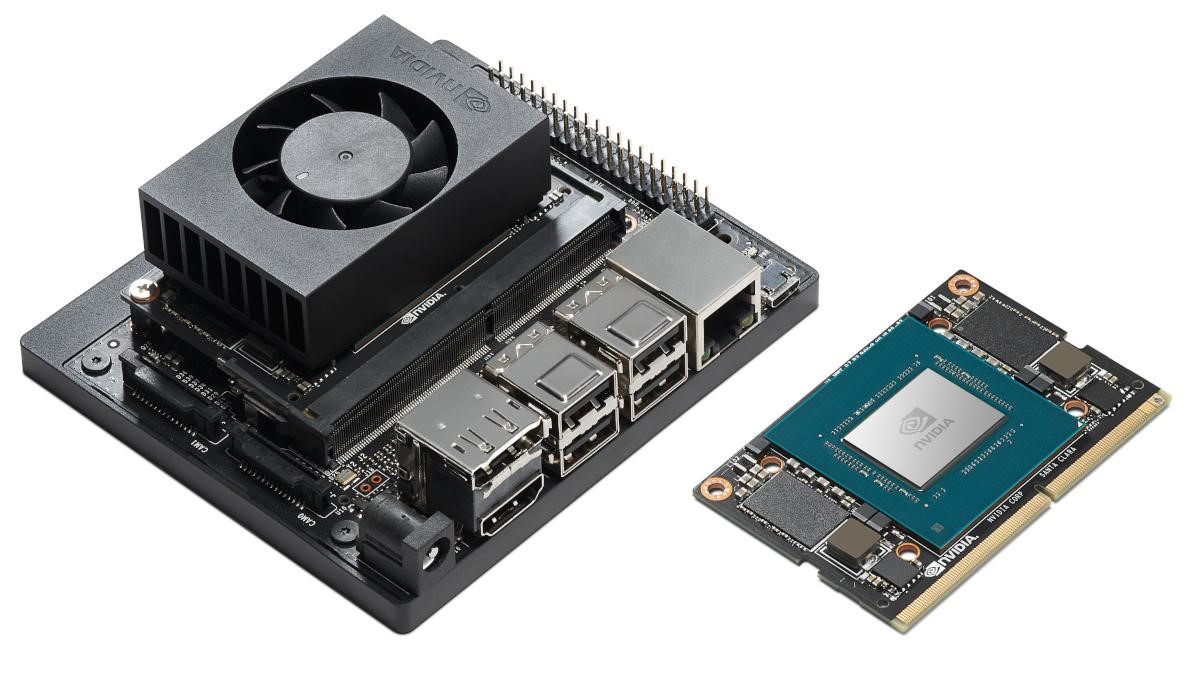
\includegraphics[scale=0.35]{figs/chapter3/nx.jpg}
    \caption{SoC Nvidia Jetson Xavier NX.}
    \label{fig:nx}
\end{figure}

\newsection{Operating System}
\indent Appare chiaro dall'architettura illustrata finora come in questo progetto si sia reso necessario interagire con l'hardware, a basso livello, e contemporaneamente sviluppare un software stratificato che lo pilotasse e implementasse opportune logiche decisionali. Per far questo, è apparsa da subito chiara la necessità di un sistema operativo che consentisse di operare facilmente ad ogni livello. Le soluzioni Jetson, basate su architettura ARM, sono studiate per essere utilizzate con il sistema operativo Linux, che soddisfa totalmente tali requisiti operativi. Ciò nonostante, è stato necessario un lavoro di configurazione ad-hoc a partire dall'installazione fornita da Nvidia per meglio adattarla al presente caso d'uso e consentire l'integrazione del resto dell'hardware e degli strumenti software impiegati.\\
L'installazione di default offerta da Nvidia è costituita dalla distribuzione Ubuntu Linux 18.04 con kernel 4.9 PREEMPT\footnote{La versione PREEMPT del kernel Linux è caratterizzata da latenze ridotte, in quanto fatta eccezione per alcune sezioni molto critiche esso risulta sempre interrompibile.}, racchiusa in una collezione di package denominata \emph{Linux 4 Tegra}. Si tratta di un'installazione stabile e testata, dotata di un set di pacchetti e librerie più limitato rispetto alle versioni base ma di tutti i driver necessari ad usare l'hardware presente sulla board. La prima strada intrapresa è stata quella dell'aggiornamento a Ubuntu 20.04, ancora non standardizzata da Nvidia, lungo la quale sono sorti diversi problemi legati all'aggiornamento delle librerie grafiche pian piano risolti. Successivamente, allo scopo di aumentare ancora di più la responsività e la predicibilità del sistema, è stata tentata la costruzione di un'installazione stabile con kernel 4.9 PREEMPT RT\footnote{La versione PREEMPT RT del kernel, ottenuta mediante l'applicazione di un set di patches prima della compilazione, è caratterizzata dall'interrompibilità totale in qualunque punto e dall'assenza di primitive di sincronizzazione di tipo \emph{locking}.}. Nonostante ripetuti tentativi di ricompilazione del kernel e di aggiornamento del sistema, sono sempre stati rilevati dei problemi di compatibilità con i driver e le librerie offerti da Nvidia, e gli incrementi prestazionali ricavati sono stati giudicati eccessivamente ridotti; oltre a ciò, si sospetta che l'aver reso interamente interrompibili anche i driver della GPU abbia reso meno efficienti alcuni algoritmi implementati su di essa. Per tali ragioni questa strada è stata abbandonata, e l'installazione PREEMPT è stata consolidata con delle performance accettabili sia sul fronte della varianza dei timer ad alta risoluzione, sia su quello dell'affidabilità delle schedulazioni soft real-time implementate mediante lo scheduler di sistema. Si ritiene, come si mostrerà, che un tale sistema sia adatto anche all'implementazione di loop di controllo veloci con campionamenti non inferiori al singolo millisecondo, naturalmente quando non si è complessivamente vicini ai suoi limiti di carico. Per misurare le latenze e valutare le prestazioni complessive è stata impiegata la utility \emph{cyclictest}\footnote{https://wiki.linuxfoundation.org/realtime/documentation/howto/tools/cyclictest/start}, una cui esecuzione è mostrata a titolo di esempio nel listato seguente.\vfill\newpage

\begin{lstlisting}[language=bash, caption=Esempio di benchmark del SoC montato sul drone eseguito con la utility \emph{cyclictest}.]
nxdrone:~$ sudo cyclictest -m -p98 --smp
# /dev/cpu_dma_latency set to 0us
policy: fifo: loadavg: 0.33 0.61 0.32 1/381 10460          

T: 0 (10428) P:98 I:1000 C:   3365 Min:      7 Act:   30 Avg:   19 Max:     147
T: 1 (10431) P:98 I:1500 C:   2241 Min:      7 Act:   21 Avg:   22 Max:     294
T: 2 (10432) P:98 I:2000 C:   1680 Min:      8 Act:   16 Avg:   27 Max:     352
T: 3 (10434) P:98 I:2500 C:   1343 Min:      8 Act:   23 Avg:   22 Max:     155
T: 4 (10435) P:98 I:3000 C:   1118 Min:      7 Act:   30 Avg:   25 Max:     147
T: 5 (10436) P:98 I:3500 C:    958 Min:      9 Act:   22 Avg:   24 Max:     319
\end{lstlisting}

Da tale esecuzione si evince come le latenze siano comunque contenute, in media nell'ordine delle decine di microsecondi, con dei picchi attesi data la configurazione del sistema, dipendenti dal carico ma comunque mai eccessivi.
\clearpage

\newsection{Software}
\indent La realizzazione di un drone autonomo in grado di eseguire deterministicamente e con precisione i task specificati nel regolamento del Contest ha posto come prima problematica la scelta di un'architettura software efficiente, e anche comoda da usare sia durante lo sviluppo che in fase di testing. Per ragioni che a questo punto dovrebbero risultare evidenti, all'installazione di Linux descritta nella sezione precedente è stato aggiunto il middleware ROS 2 versione Foxy Fitzroy.\\
I vari task necessari al compimento di una missione sono stati suddivisi in livelli:
\begin{itemize}
    \item a basso livello: comunicazione con il controllore di volo Pixhawk per invio comandi, ricezione di feedback e informazioni di stato e campionamento dell'odometria;
    \item ad un livello intermedio: comunicazione con le camere per configurarle e ricevere i frame da cui estrarre informazioni;
    \item ad un livello più alto: algoritmi di esplorazione, navigazione e precision landing, logica decisionale e comunicazione con la Ground Control Station.
\end{itemize}
Naturalmente ciascuno di questi moduli è stato realizzato come package ROS 2, comprendente uno o più nodi secondo le necessità. Ciò che li differenzia è la diversa modalità operativa: i nodi appartenenti al livello più basso hanno quasi sempre callbacks in esecuzione o eventi da gestire, e fanno un uso preponderante dei messaggi; quelli appartenenti al livello intermedio svolgono lavoro non appena sono disponibili nuovi dati da processare, pubblicando i risultati sempre sotto forma di messaggi; infine, le logiche e gli algoritmi di più alto livello sono attivati solo quando richiesto, ossia in momenti specifici della missione, e sono pertanto invocati sempre mediante dei servizi. Le interfacce che si sono dovute definire ad-hoc sono state raccolte nel package \emph{afg\_interfaces}. Data la criticità di alcune operazioni, nonché la necessità di lavorare talvolta a diretto contatto con l'hardware a disposizione, l'unico linguaggio di programmazione impiegato è stato il C++. Nel resto di questa sezione si procederà dunque a descrivere nel dettaglio tutti i packages e i nodi che compongono l'architettura, secondo il naturale ordinamento gerarchico appena illustrato. Una rappresentazione complessiva di tale architettura è offerta in Figura \ref{fig:nodesgraph}: tale schema è stato ricavato con il tool rqt\_graph ed evidenzia tutti i nodi attivi sul drone e la GCS, nonché i topic su cui alcuni di essi si scambiano messaggi. Sono assenti i servizi, non rappresentabili graficamente da rqt\_graph, nonché i topic esposti dal microRTPS Agent su cui viaggiano le comunicazioni da e verso il controllore di volo: tutti questi elementi saranno illustrati più in dettaglio nel seguito, assieme a degli schemi relativi ai singoli packages.

\begin{figure}
    \centering
    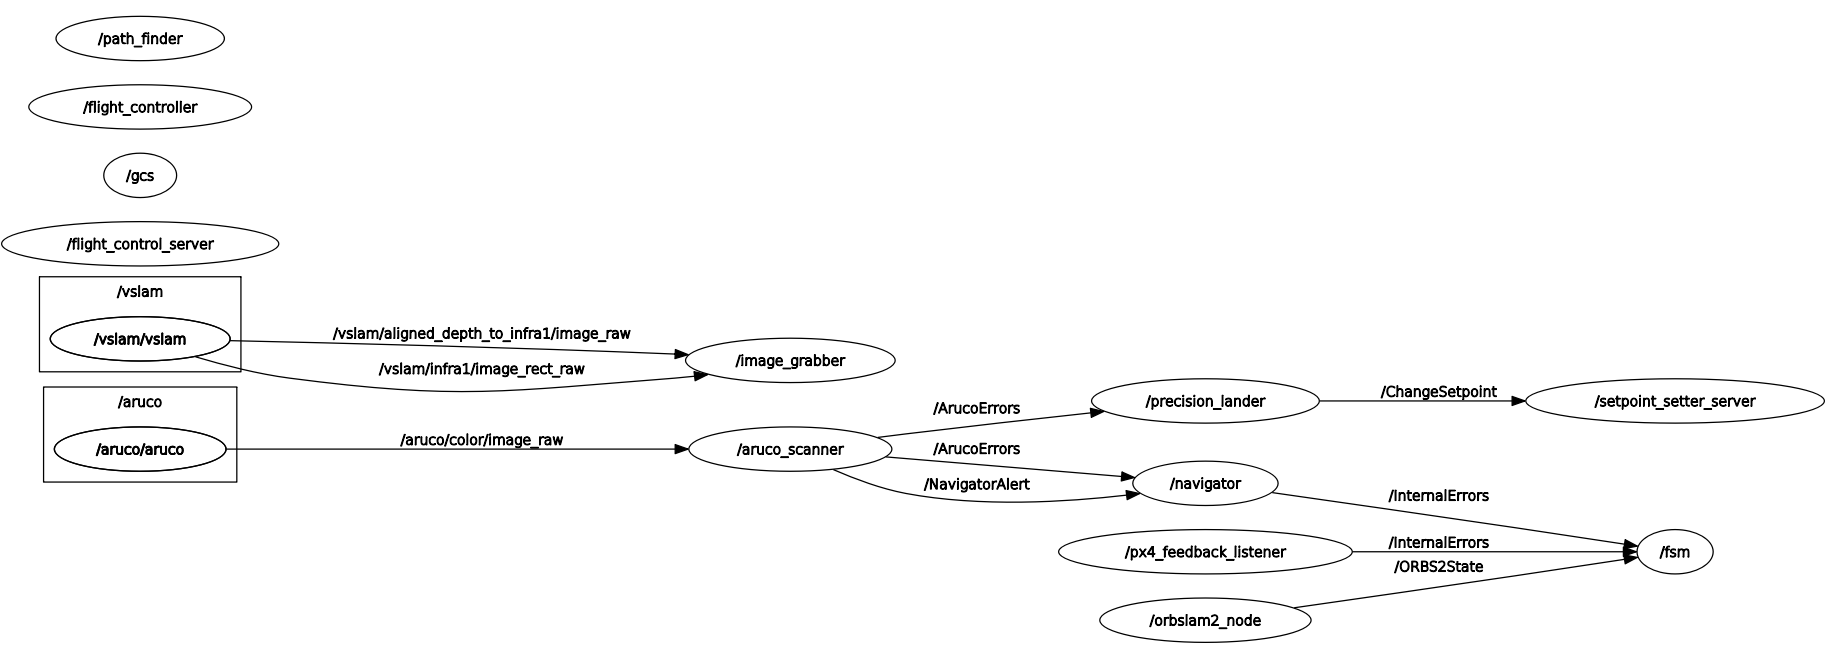
\includegraphics[width=\textwidth]{figs/chapter3/nodesgraph.png}
    \caption{Schema complessivo di nodi e topic attivi su drone e GCS.}
    \label{fig:nodesgraph}
\end{figure}

\newsubsection{Flight Control}
\indent Il primo livello dell'architettura software, direttamente al di sopra del firmware PX4 in esecuzione nel controllore di volo Pixhawk, è rappresentato dal package \emph{Flight Control}. I compiti svolti da questo programma, e ripartiti tra un totale di quattro nodi, sono i seguenti:
\begin{itemize}
    \item invio di comandi a PX4 per l'esecuzione di operazioni relative al volo quali armamento, disarmamento, decollo e atterraggio, quando richiesto da altri nodi o da un operatore;
    \item invio periodico a PX4 di setpoint di posizione o velocità da inseguire;
    \item parsing delle richieste formulate dagli altri nodi per cambiare i setpoint da inviare a PX4, al fine di spostare il drone nell'ambiente;
    \item ricezione e parsing di feedback da PX4 relativi ai comandi operativi, nonché allo stato di basso livello del drone, e degli stessi messaggi di log di PX4.
\end{itemize}

\begin{figure}
    \centering
    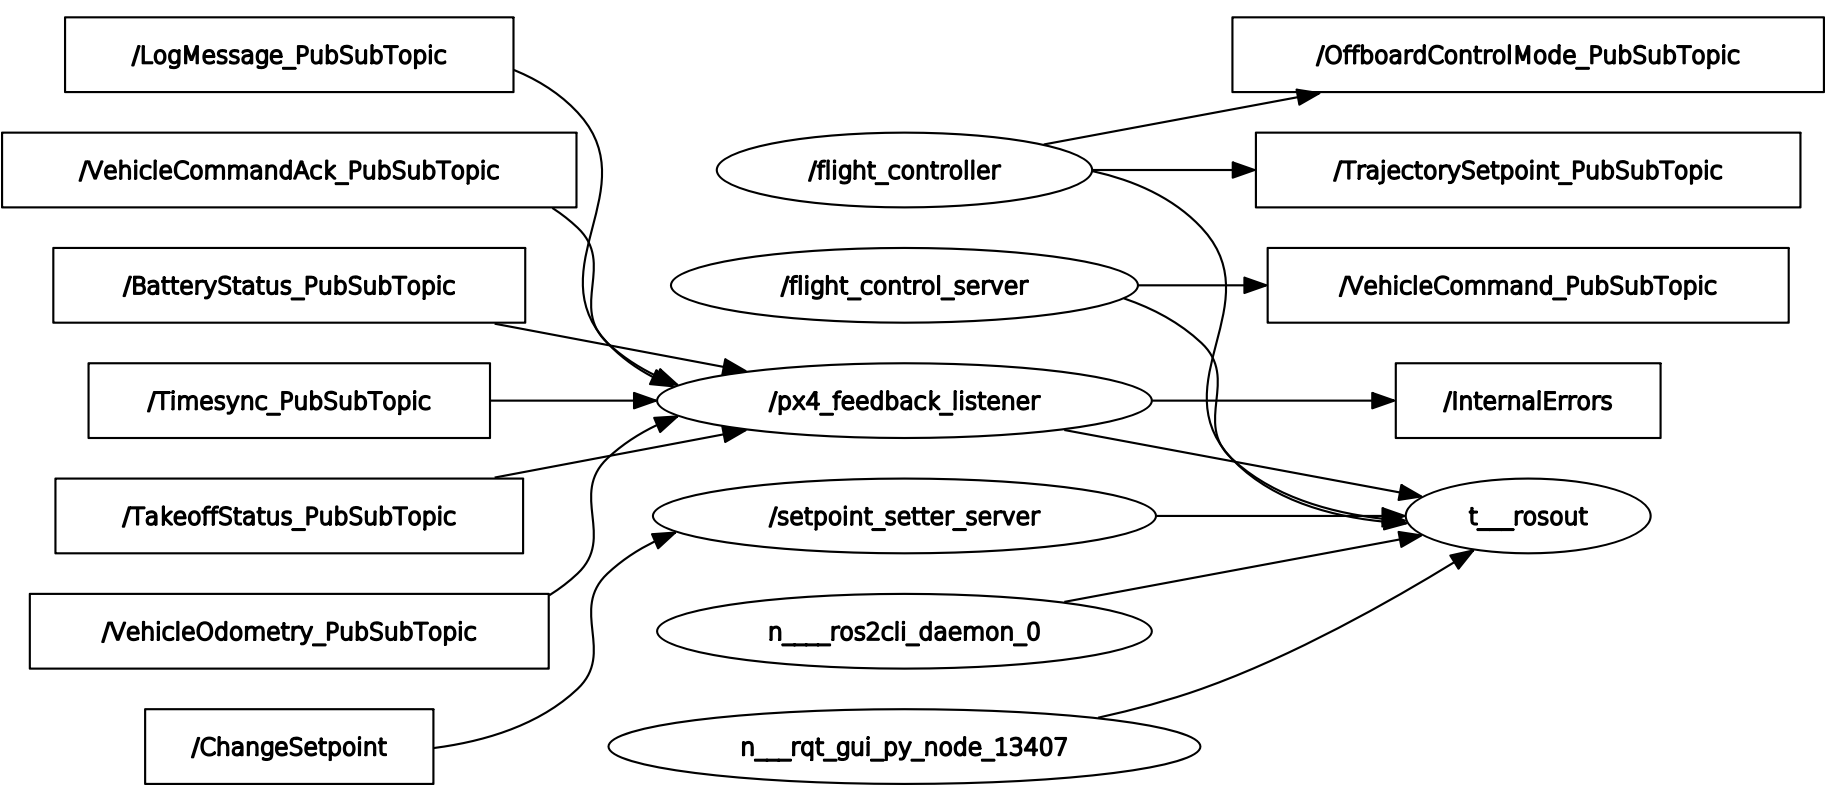
\includegraphics[width=\textwidth]{figs/chapter3/fctrl.png}
    \caption{Schema riassuntivo di nodi e topic del package \emph{Flight Control}.}
    \label{fig:fctrl}
\end{figure}

\newsection{Realizzazione}
\indent
